\documentclass{beamer}
\usepackage[utf8]{inputenc}

\usetheme{Madrid}
\usecolortheme{default}
\usepackage{amsmath}
\usepackage{amssymb,amsfonts,amsthm}
\usepackage{txfonts}
\usepackage{tkz-euclide}
\usepackage{listings}
\usepackage{adjustbox}
\usepackage{array}
\usepackage{tabularx}
\usepackage{gvv}
\usepackage{lmodern}
\usepackage{circuitikz}
\usepackage{tikz}
\usepackage{graphicx}

\setbeamertemplate{page number in head/foot}[totalframenumber]

\usepackage{tcolorbox}
\tcbuselibrary{minted,breakable,xparse,skins}



\definecolor{bg}{gray}{0.95}
\DeclareTCBListing{mintedbox}{O{}m!O{}}{%
  breakable=true,
  listing engine=minted,
  listing only,
  minted language=#2,
  minted style=default,
  minted options={%
    linenos,
    gobble=0,
    breaklines=true,
    breakafter=,,
    fontsize=\small,
    numbersep=8pt,
    #1},
  boxsep=0pt,
  left skip=0pt,
  right skip=0pt,
  left=25pt,
  right=0pt,
  top=3pt,
  bottom=3pt,
  arc=5pt,
  leftrule=0pt,
  rightrule=0pt,
  bottomrule=2pt,
  toprule=2pt,
  colback=bg,
  colframe=orange!70,
  enhanced,
  overlay={%
    \begin{tcbclipinterior}
    \fill[orange!20!white] (frame.south west) rectangle ([xshift=20pt]frame.north west);
    \end{tcbclipinterior}},
  #3,
}
\lstset{
    language=C,
    basicstyle=\ttfamily\small,
    keywordstyle=\color{blue},
    stringstyle=\color{orange},
    commentstyle=\color{green!60!black},
    numbers=left,
    numberstyle=\tiny\color{gray},
    breaklines=true,
    showstringspaces=false,
}
\title{2.4.20}
\date{31st August, 2025}
\author{Vishwambhar - EE25BTECH11025}

\begin{document}

\frame{\titlepage}
\begin{frame}{Question}
Find the value of $\lambda$ such that the vectors $\vec{a}=2\vec{i}+\lambda\vec{j}+\vec{k}$ and $\vec{b}=\vec{i}+2\vec{j}+3\vec{k}$ are orthogonal.
\end{frame}

\begin{frame}{Given Vectors}
\begin{align}
    \vec{a}=\myvec{2\\\lambda\\1},
    \vec{b}=\myvec{1\\2\\3}
\end{align}
\end{frame}

\begin{frame}{Finding Lambda$\brak{\lambda}$}
For two vectors to be orthogonal their dot product should be equal to zero which is equal to product of transpose of column matrix $\vec{a}$ and column matrix $\vec{b}$:
\begin{align}
    \vec{a}^T\vec{b}=0\\
    \myvec{2&\lambda&1}\myvec{1\\2\\3}=0\\
    2+2\lambda+3=0\\
    \lambda=\brak{\frac{-5}{2}}
\end{align}
\end{frame}

\begin{frame}{Final vectors}
    Therefore, the final vectors are:
\begin{align}
    \vec{a}=\myvec{2\\\brak{\frac{-5}{2}}\\1}\\
    \vec{b}=\myvec{1\\2\\3}
\end{align}
\end{frame}

\begin{frame}[fragile]
    \frametitle{C Code}
    \begin{lstlisting}
#include <stdio.h>
void make_data(double *points){
    points[0] = 1;
    points[1] = 2;
    points[2] = 3;
    double lambda_val;
    lambda_val = -2.5;
    points[3] = lambda_val;
}
    \end{lstlisting}
\end{frame}

\begin{frame}[fragile]
    \frametitle{Python Code 1}
    \begin{lstlisting}
import ctypes as ct
def give_data():
    lib = ct.CDLL("./problem.so")
    entry = ct.c_double*4
    lib.make_data.argtypes = [ct.POINTER(ct.c_double)]
    data = entry()
    lib.make_data(data)
    return data[1], data[3], data[0], data[0], data[1], data[2]
    \end{lstlisting}
\end{frame}

\begin{frame}[fragile]
    \frametitle{Python Code 2}
    \begin{lstlisting}
import numpy as np
import matplotlib.pyplot as plt
from call import give_data
Ax, Ay, Az, Bx, By, Bz = give_data()
lambda_val = -2.5
a = np.array([Ax, Ay, Az])   
b = np.array([Bx, By, Bz])   
fig = plt.figure()
ax = fig.add_subplot(111, projection='3d')
ax.quiver(0, 0, 0, a[0], a[1], a[2], color='r', label='Vector a')
ax.quiver(0, 0, 0, b[0], b[1], b[2], color='b', label='Vector b')
    \end{lstlisting}
\end{frame}

\begin{frame}[fragile]
    \frametitle{Python Code 2}
    \begin{lstlisting}
ax.text(a[0], a[1], a[2], 'a', fontsize=12)
ax.text(b[0], b[1], b[2], 'b', fontsize=12)
ax.set_xlabel('X')
ax.set_ylabel('Y')
ax.set_zlabel('Z')
ax.set_title("Orthogonal Vectors a and b")
ax.legend()
plt.savefig("../figs/plot.png")
plt.show()
    \end{lstlisting}
\end{frame}

\begin{frame}{Plot}
    \begin{figure}
        \centering
        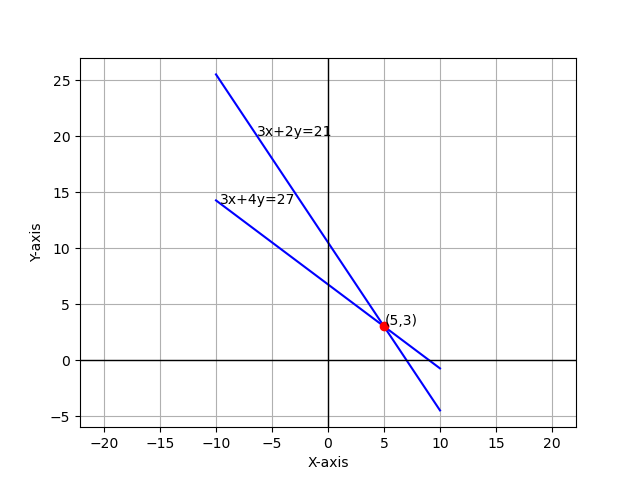
\includegraphics[width=0.5\columnwidth]{../figs/plot.png}
        \caption{Plot of orthogonal vectors $\vec{a}$ and $\vec{b}$.}
        \label{fig:fig}
    \end{figure}
\end{frame}
\end{document}
